\documentclass[11pt,twoside,a4paper]{article}

\begin{document}

Traditional opposition between \textit{factual} and \textit{normative}.

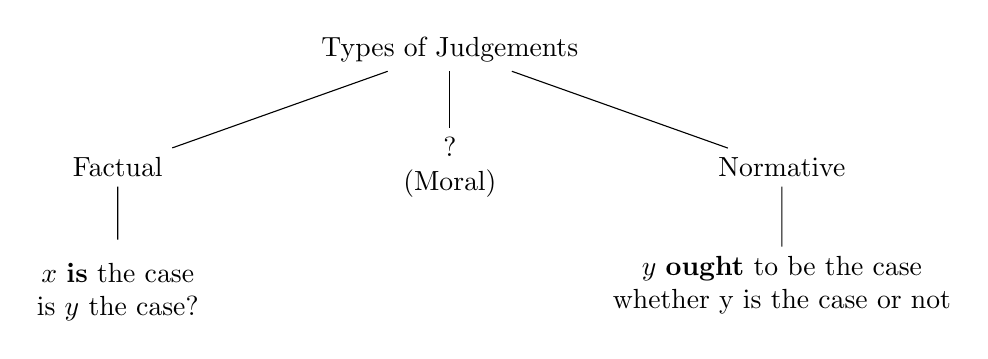
\begin{tikzpicture}[every node/.style={align=center},level 1/.style={sibling distance=12em},level 2/.style={sibling distance=35mm}, level 3/.style={sibling distance=15mm} level 4/.style={sibling distance=30mm}
]
\node {Types of Judgements}
[sibling distance=6cm]
child { node {Factual} 
    child { node { \\ \textit{$x$} \textbf{is} the case \\ is \textit{$y$} the case?}}} % <- end fact
child { node {? \\ (Moral)} } % <- end any
child { node {Normative} 
    child{ node {\textit{$y$} \textbf{ought} to be the case \\ whether y is the case or not}}} %<-end cognition
; %<-end node
\end{tikzpicture}

\end{document}